\chapter{A catálise}\label{ch:g12:catalysis}

Um frasco de água oxigenada fica meses no armário do banheiro sem mudar.
Derramada num joelho ralado, ela espuma na hora: alguma coisa do sangue
faz com que ela se decomponha em segundos em água e gás oxigênio. Essa
coisa não é consumida, e não aparece na equação da reação. Ela é um
\omterm{def:g12:catalysis:catalyst}{catalisador}. Os \omterm{def:g12:catalysis:catalyst}{catalisadores} tornam possível a maior parte da indústria
química, limpam o escapamento dos carros e comandam todas as reações da
vida.

\begin{recall}
A velocidade de uma reação e os \omterm{def:g12:reaction-rates:kinetic-factor}{fatores cinéticos} que a modificam
(\cref{ch:g12:reaction-rates}). Um mecanismo é uma série de \omterm{def:g12:curly-arrows:mechanism}{etapas
elementares}, que passam por intermediários (\cref{ch:g12:curly-arrows}).
\end{recall}

\section{O que é um catalisador}

\begin{definition}[Catalisador, catálise]\label{def:g12:catalysis:catalyst}
Um \emph{catalisador}\index{catalisador} é uma espécie que torna uma
reação mais rápida sem ser consumida: ele participa do mecanismo, mas é
devolvido, intacto, no final, e não aparece na equação global. A
aceleração de uma reação por um catalisador é a
\emph{catálise}\index{catalise@catálise}.
\end{definition}

\begin{proposition}[Um catalisador muda o caminho, não o destino]\label{prop:g12:catalysis:path}
Um \omterm{def:g12:catalysis:catalyst}{catalisador} abre um outro mecanismo, cujas barreiras de energia são
mais baixas que a da reação não catalisada, de modo que uma parte maior
dos encontros entre partículas dá certo. Ele não muda os produtos
formados, nem o \omterm{def:g10:reaction-progress-table:system}{estado final} alcançado; ele só o alcança mais cedo.
\end{proposition}

\begin{proof}
Admitido: o perfil é estudado no volume do primeiro ano da universidade.
Que o \omterm{def:g10:reaction-progress-table:system}{estado final} não muda decorre do fato de o \omterm{def:g12:catalysis:catalyst}{catalisador} ser
devolvido: a reação global, \omterm{def:g7:chemical-reactions:reactant}{reagentes} e produtos, é a mesma.
\end{proof}

\begin{omfigure}
\begin{minipage}{0.49\linewidth}
\begin{tikzpicture}
\begin{axis}[width=\linewidth, height=5.4cm, xmin=0, xmax=1, ymin=-60,
    ymax=110, xtick=\empty, ytick=\empty, axis lines*=left,
    xlabel={avanço da reação}, ylabel={energia},
    label style={font=\small}, legend style={font=\scriptsize,
    at={(0.02,0.99)}, anchor=north west, draw=none}, legend cell align=left]
  \addplot[very thick, omDef] table[x=s, y=Eu] {figdata/out/grade-12-catalysis-a.dat};
  \addplot[very thick, omProp] table[x=s, y=Ec] {figdata/out/grade-12-catalysis-a.dat};
  \legend{sem catalisador, com catalisador}
  \node[font=\scriptsize, anchor=north west] at (axis cs:0.02,-4) {reagentes};
  \node[font=\scriptsize, anchor=south east] at (axis cs:0.99,-36) {produtos};
\end{axis}
\end{tikzpicture}
\end{minipage}\hfill
\begin{minipage}{0.49\linewidth}
\begin{tikzpicture}
\begin{axis}[width=\linewidth, height=5.4cm, xmin=0, xmax=60, ymin=0,
    ymax=80, xlabel={$t$ (\si{min})}, ylabel={\ce{O2} liberado (\si{mL})},
    axis lines*=left, ymajorgrids, grid style={gray!20},
    tick label style={font=\scriptsize}, label style={font=\small},
    legend style={font=\scriptsize, at={(0.98,0.03)}, anchor=south east,
    draw=none}, legend cell align=left]
  \addplot[very thick, omDef] table[x=t, y=Vu] {figdata/out/grade-12-catalysis-b.dat};
  \addplot[very thick, omProp] table[x=t, y=Vc] {figdata/out/grade-12-catalysis-b.dat};
  \legend{sem catalisador, com catalisador}
\end{axis}
\end{tikzpicture}
\end{minipage}

{\small À esquerda: a energia ao longo da reação; o caminho catalisado
passa por um intermediário e por duas barreiras mais baixas. À direita:
o gás oxigênio liberado por uma solução de peróxido de hidrogênio; o
\omterm{def:g12:catalysis:catalyst}{catalisador} acelera a reação, mas o volume final é o mesmo. (Curvas de
modelo.)}
\end{omfigure}

\section{A catálise homogênea}

\begin{definition}[Catálise homogênea e heterogênea]\label{def:g12:catalysis:homogeneous}
A \omterm{def:g12:catalysis:catalyst}{catálise} é uma \emph{catálise homogênea}\index{catalise homogenea@catálise homogênea}
quando o \omterm{def:g12:catalysis:catalyst}{catalisador} está na mesma fase que os \omterm{def:g7:chemical-reactions:reactant}{reagentes} (por exemplo,
dissolvido com eles), e uma \emph{catálise
heterogênea}\index{catalise heterogenea@catálise heterogênea} quando ele está em outra fase,
em geral um sólido cuja superfície os \omterm{def:g7:chemical-reactions:reactant}{reagentes} alcançam a partir de um
gás ou de um líquido.
\end{definition}

\begin{example}[Os íons iodeto e o peróxido de hidrogênio]\label{ex:g12:catalysis:iodide}
O peróxido de hidrogênio se decompõe muito devagar sozinho:
\ce{2H2O2 -> 2H2O + O2}. Com um pouco de iodeto de potássio dissolvido
nele, ele espuma na hora. O \omterm{def:g9:ions:ion}{íon} iodeto abre um caminho em duas etapas:
\[
  \ce{H2O2 + I- -> H2O + IO-}, \qquad
  \ce{H2O2 + IO- -> H2O + O2 + I-} .
\]
Somadas, as duas etapas devolvem \ce{2H2O2 -> 2H2O + O2}: o \omterm{def:g9:ions:ion}{íon} iodeto,
consumido na primeira etapa e devolvido na segunda, é o \omterm{def:g12:catalysis:catalyst}{catalisador}; o
\omterm{def:g9:ions:ion}{íon} \ce{IO-} é um intermediário.
\end{example}


\begin{example}[Os íons ferro(III)]\label{ex:g12:catalysis:iron}
Os \omterm{def:g9:ions:ion}{íons} ferro(III) também catalisam a decomposição, por meio do par
\ce{Fe^{3+}}/\ce{Fe^{2+}} (\cref{ch:g11:redox}): primeiro eles oxidam o
peróxido de hidrogênio, \ce{2Fe^{3+} + H2O2 -> 2Fe^{2+} + O2 + 2H+},
depois os \omterm{def:g9:ions:ion}{íons} ferro(II) formados são oxidados de volta por mais
peróxido de hidrogênio, \ce{2Fe^{2+} + H2O2 + 2H+ -> 2Fe^{3+} + 2H2O}. A
cor laranja-clara da solução fica esverdeada enquanto o gás é liberado,
e depois volta quando o peróxido de hidrogênio acaba: sinal de que o
\omterm{def:g12:catalysis:catalyst}{catalisador} participa e é regenerado.
\end{example}

\section{A catálise heterogênea}

Muitos \omterm{def:g12:catalysis:catalyst}{catalisadores} industriais são sólidos: \omterm{def:g9:periodic-table-first-look:metal}{metais} como a platina, o
paládio, o níquel ou o ferro, ou óxidos. A reação acontece na sua
superfície, em três etapas: as \omterm{def:g7:atoms-and-molecules:molecule}{moléculas} dos \omterm{def:g7:chemical-reactions:reactant}{reagentes} ficam retidas na
superfície (adsorvidas), onde as suas ligações se enfraquecem; elas
reagem ali; os produtos deixam a superfície, que fica livre para novas
\omterm{def:g7:atoms-and-molecules:molecule}{moléculas}. Por isso, um \omterm{def:g12:catalysis:catalyst}{catalisador} é fabricado com a maior superfície
possível: pó fino, ou uma camada fina sobre um suporte poroso.

\begin{omfigure}
\begin{tikzpicture}[font=\small]
  \foreach \x in {0,4.2,8.4} {
    \fill[black!25] (\x,0) rectangle (\x+3.4,0.35);
    \foreach \i in {0,1,2,3,4,5,6,7} \shade[ball color=black!35] (\x+0.21+\i*0.425,0.35) circle (0.2);
  }
  % 1. adsorption
  \node[aH, minimum size=3.2mm] at (0.9,0.75) {};
  \node[aH, minimum size=3.2mm] at (1.3,0.75) {};
  \node[aH, minimum size=3.2mm] (h1) at (2.2,1.8) {};
  \node[aH, minimum size=3.2mm] (h2) at (2.6,1.8) {};
  \draw[bond, line width=1.2pt] (h1.east) -- (h2.west);
  \draw[->, omProp, thick] (2.4,1.55) -- (2.0,1.0);
  \node[anchor=north, align=center] at (1.7,-0.1) {1. adsorção:\\ a ligação \ce{H-H} se rompe};
  % 2. reaction on the surface
  \node[aC] (c1) at (5.5,1.05) {}; \node[aC] (c2) at (6.2,1.05) {};
  \draw[bond, line width=1.4pt] (c1) -- (c2);
  \node[aH, minimum size=3.2mm] at (5.3,0.75) {};
  \node[aH, minimum size=3.2mm] at (6.6,0.75) {};
  \node[anchor=north, align=center] at (5.9,-0.1) {2. os átomos H se juntam\\ à molécula adsorvida};
  % 3. desorption
  \node[aC] (c3) at (9.6,1.8) {}; \node[aC] (c4) at (10.3,1.8) {};
  \draw[bond, line width=1.4pt] (c3) -- (c4);
  \foreach \a/\c in {150/c3,210/c3,90/c3,30/c4,-30/c4,90/c4}
    \node[aH, minimum size=2.8mm] at ($(\c)+(\a:0.42)$) {};
  \draw[->, omProp, thick] (11.0,1.2) -- (11.0,2.2);
  \node[anchor=north, align=center] at (10.1,-0.1) {3. o produto\\ deixa a superfície};
\end{tikzpicture}

{\small O hidrogênio se adicionando ao eteno numa superfície metálica:
adsorção, reação, dessorção. O \omterm{def:g9:periodic-table-first-look:metal}{metal} é devolvido intacto.}
\end{omfigure}

\begin{example}[O conversor catalítico]\label{ex:g12:catalysis:converter}
O escapamento de um motor a gasolina contém monóxido de carbono e
monóxido de nitrogênio, ambos tóxicos, e \omterm{def:g4:what-a-fire-needs:fuel}{combustível} não queimado. No
conversor catalítico, uma colmeia de cerâmica revestida de platina e de
ródio, eles reagem na superfície do \omterm{def:g9:periodic-table-first-look:metal}{metal}:
\[
  \ce{2CO + 2NO -> 2CO2 + N2} ,
\]
e os hidrocarbonetos queimam, dando dióxido de carbono e água. Os gases
atravessam o conversor numa fração de segundo, depressa demais para
qualquer reação sem \omterm{def:g12:catalysis:catalyst}{catalisador}.
\end{example}

\begin{omfigure}
\begin{tikzpicture}[font=\small]
  \fill[black!12, draw=black!60, rounded corners=6pt] (0,0) rectangle (6,2.4);
  \foreach \x in {0.3,0.6,0.9,1.2,1.5,1.8,2.1,2.4,2.7,3.0,3.3,3.6,3.9,4.2,4.5,4.8,5.1,5.4,5.7} \draw[black!35] (\x,0.2) -- (\x,2.2);
  \foreach \y in {0.5,0.9,1.3,1.7,2.1} \draw[black!35] (0.2,\y) -- (5.8,\y);
  \fill[black!40] (-1.4,0.9) rectangle (0,1.5);
  \fill[black!40] (6,0.9) rectangle (7.4,1.5);
  \draw[->, very thick, omThm] (-2.6,1.2) -- (-1.5,1.2);
  \node[anchor=east, align=right, omThm] at (-2.7,1.2) {\ce{CO}, \ce{NO},\\ hidrocarbonetos};
  \draw[->, very thick, omMeth] (7.5,1.2) -- (8.6,1.2);
  \node[anchor=west, align=left, omMeth] at (8.7,1.2) {\ce{CO2}, \ce{N2},\\ \ce{H2O}};
  \node[align=center, fill=white, inner sep=2pt] at (3,1.2) {colmeia de cerâmica\\ revestida de Pt e Rh};
\end{tikzpicture}

{\small Um conversor catalítico, cortado no sentido do comprimento:
milhares de canais finos dão aos gases do escapamento uma enorme
superfície revestida de \omterm{def:g9:periodic-table-first-look:metal}{metal}.}
\end{omfigure}

\begin{omfigure}
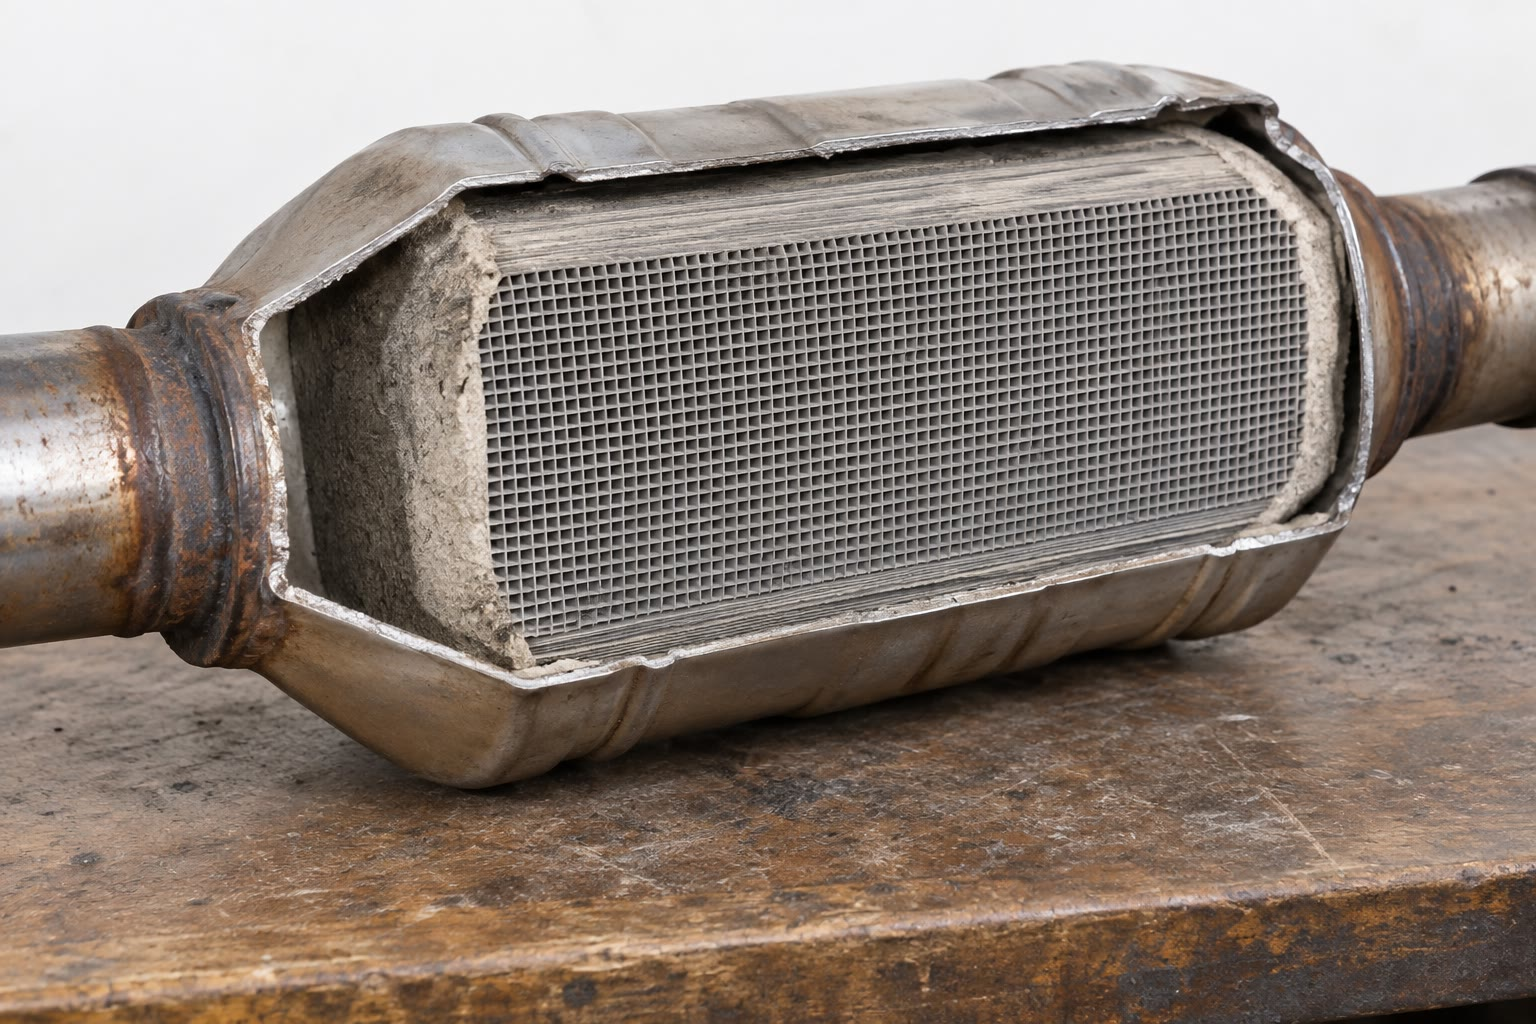
\includegraphics[width=0.45\linewidth]{images/book1/ai/g12-catalytic-converter.jpg}

{\small Um conversor catalítico aberto: o núcleo em colmeia.}
\end{omfigure}

\begin{history}[Haber, Bosch e a amônia]
% ledger: haber:T, haber:p, nh3:world-2024
No início do século XX, o químico Fritz Haber descobriu como combinar o
nitrogênio do \omterm{def:g4:air-a-mixture-of-gases:air}{ar} com o hidrogênio, \ce{N2 + 3H2 -> 2NH3}, sobre um
\omterm{def:g12:catalysis:catalyst}{catalisador} à base de ferro, e o engenheiro Carl Bosch transformou isso
num processo industrial. Ele ainda funciona hoje a 400--\qty{500}{\celsius}
e 150--\qty{250}{atm}. Em 2024, o mundo fabricou amônia contendo cerca de
150 milhões de toneladas de nitrogênio, a maior parte para fertilizantes:
uma grande parte do nitrogênio dos alimentos que comemos passou por um
\omterm{def:g12:catalysis:catalyst}{catalisador} desses.
\end{history}

\section{As enzimas}

\begin{definition}[Enzima]\label{def:g12:catalysis:enzyme}
Uma \emph{enzima}\index{enzima} é uma proteína fabricada por um ser vivo
que catalisa uma reação da sua química. As enzimas são muito eficientes
e muito específicas: cada uma só se encaixa em algumas \omterm{def:g7:atoms-and-molecules:molecule}{moléculas}, e elas
funcionam melhor numa faixa estreita de temperatura e de acidez.
\end{definition}

\begin{example}[A catalase]\label{ex:g12:catalysis:catalase}
O peróxido de hidrogênio se forma nas células como subproduto, e é
nocivo para elas. A \omterm{def:g12:catalysis:enzyme}{enzima} catalase, presente no sangue, no fígado e em
muitos tecidos vegetais, o decompõe em água e gás oxigênio a uma
velocidade enorme: é a espuma num joelho ralado, ou numa fatia de batata
crua. A batata cozida não faz espuma: o aquecimento destruiu a forma da
\omterm{def:g12:catalysis:enzyme}{enzima}.
\end{example}

\begin{omfigure}
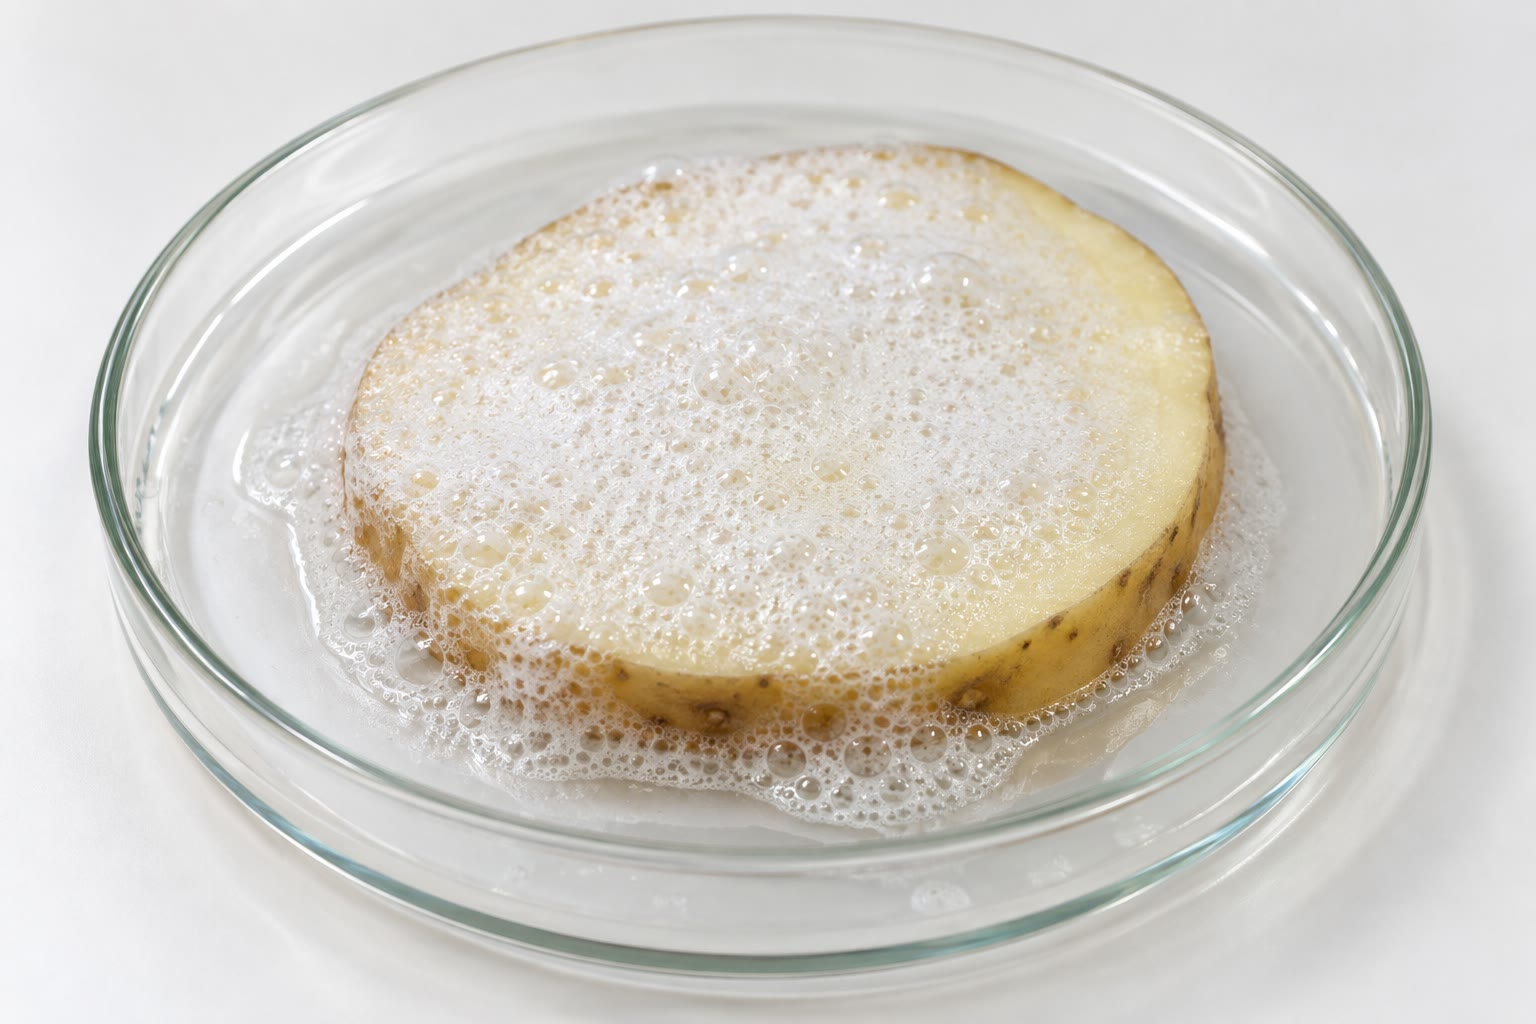
\includegraphics[width=0.45\linewidth]{images/book1/ai/g12-potato-peroxide.jpg}

{\small Água oxigenada numa fatia de batata crua: a catalase em ação.}
\end{omfigure}

\section{A seletividade}

\begin{definition}[Catalisador seletivo]\label{def:g12:catalysis:selective}
Quando os mesmos \omterm{def:g7:chemical-reactions:reactant}{reagentes} podem dar várias reações, um
\emph{catalisador seletivo}\index{catalisador seletivo} acelera uma delas
muito mais que as outras, e assim decide que produtos se formam.
\end{definition}

\begin{example}[Dois destinos para o etanol]\label{ex:g12:catalysis:ethanol}
O vapor de etanol quente, passado sobre alumina, perde água e dá eteno,
\ce{C2H5OH -> C2H4 + H2O} (uma \omterm{def:g12:curly-arrows:categories}{eliminação}); passado sobre cobre quente,
ele perde hidrogênio e dá etanal, \ce{C2H5OH -> CH3CHO + H2}. O mesmo
\omterm{def:g7:chemical-reactions:reactant}{reagente}, dois \omterm{def:g12:catalysis:catalyst}{catalisadores}, dois produtos.
\end{example}

\begin{remark}[A indústria e a vida funcionam com catalisadores]\label{rem:g12:catalysis:everywhere}
A maior parte dos produtos da indústria química, dos \omterm{def:g4:what-a-fire-needs:fuel}{combustíveis} aos
\omterm{def:g8:plastics:plastic}{plásticos} e aos fertilizantes, é fabricada com \omterm{def:g12:catalysis:catalyst}{catalisadores}; encontrar
um \omterm{def:g12:catalysis:catalyst}{catalisador} mais ativo ou mais seletivo economiza energia e
resíduos. Toda reação de uma célula viva é catalisada por uma \omterm{def:g12:catalysis:enzyme}{enzima}.
\end{remark}

\begin{safety}{\ghs[0.82cm]{GHS03}\ghs[0.82cm]{GHS05}\ghs[0.82cm]{GHS07}}
% ledger: ghs:H2O2
O peróxido de hidrogênio concentrado é um \omterm{def:g11:redox:oxidant}{oxidante} forte que pode
alimentar um incêndio, queima a pele e os olhos, e é nocivo se
ingerido. As soluções diluídas do laboratório ainda exigem óculos e
luvas; a decomposição libera gás oxigênio, por isso nunca é feita num
recipiente fechado.
\end{safety}

\section{Exercícios}


\begin{exercise}[$\star$]\label{exo:g12:catalysis:1}
Na decomposição do peróxido de hidrogênio catalisada pelos \omterm{def:g9:ions:ion}{íons} iodeto,
que espécies são \omterm{def:g7:chemical-reactions:reactant}{reagentes}, quais são produtos, qual é o \omterm{def:g12:catalysis:catalyst}{catalisador},
qual é um intermediário?
\end{exercise}

\begin{exercise}[$\star$]\label{exo:g12:catalysis:2}
\omterm{def:g12:catalysis:homogeneous}{Catálise homogênea} ou heterogênea: \omterm{def:g9:ions:ion}{íons} iodeto em água oxigenada;
platina num conversor catalítico; ferro na \omterm{def:g10:synthesis-yield:synthesis}{síntese} da amônia; \omterm{def:g9:ions:ion}{íons}
ferro(III) em água oxigenada?
\end{exercise}

\begin{exercise}[$\star$]\label{exo:g12:catalysis:3}
Nos perfis de energia, que caminho tem a barreira mais alta? As energias
inicial e final são as mesmas nos dois caminhos? O que isso significa
para os produtos?
\end{exercise}

\begin{exercise}[$\star$]\label{exo:g12:catalysis:4}
Por que um \omterm{def:g12:catalysis:catalyst}{catalisador} não aparece na equação global de uma reação?
\end{exercise}

\begin{exercise}[$\star$]\label{exo:g12:catalysis:5}
Por que os \omterm{def:g12:catalysis:catalyst}{catalisadores} sólidos da indústria são usados como pós finos
ou como camadas finas sobre suportes porosos?
\end{exercise}

\begin{exercise}[$\star\star$]\label{exo:g12:catalysis:6}
Some as duas etapas da decomposição do peróxido de hidrogênio catalisada
pelo ferro(III), e mostre que os \omterm{def:g9:ions:ion}{íons} ferro e os \omterm{def:g9:ions:ion}{íons} hidrogênio se
cancelam.
\end{exercise}

\begin{exercise}[$\star\star$]\label{exo:g12:catalysis:7}
Leia as curvas do gás oxigênio liberado. Quanto tempo cada experimento
leva para liberar a metade do volume final? Por que fator o \omterm{def:g12:catalysis:catalyst}{catalisador}
encurta esse tempo?
\end{exercise}

\begin{exercise}[$\star\star$]\label{exo:g12:catalysis:8}
A gasolina com chumbo não é usada em carros equipados com conversor
catalítico: o chumbo se deposita sobre a platina e fica ali. Explique
por que isso estraga o conversor, embora a platina não seja consumida
pela reação normal.
\end{exercise}

\begin{exercise}[$\star\star$]\label{exo:g12:catalysis:9}
Um aluno mede a espuma produzida por fatias de batata em água oxigenada
a 10, 25, 37, 60 e \qty{80}{\celsius}: a espuma aumenta até cerca de
\qty{37}{\celsius}, depois diminui, e quase desaparece a
\qty{80}{\celsius}. Explique as duas partes da curva.
\end{exercise}

\begin{exercise}[$\star\star$]\label{exo:g12:catalysis:10}
Escreva a equação da reação, num conversor catalítico, entre o monóxido
de carbono e o monóxido de nitrogênio, e verifique que ela está
balanceada. Por que os dois poluentes são eliminados ao mesmo tempo?
\end{exercise}

\begin{exercise}[$\star\star$]\label{exo:g12:catalysis:11}
\qty{10.0}{mL} de água oxigenada liberam \qty{72}{mL} de gás oxigênio a
\qty{20}{\celsius} quando decompostos completamente. Calcule a
\omterm{def:g10:the-mole:amount}{quantidade de matéria} de gás oxigênio ($V_m = \qty{24.1}{L/mol}$), e
depois a concentração da solução em peróxido de hidrogênio.
\end{exercise}

\begin{exercise}[$\star\star\star$]\label{exo:g12:catalysis:12}
O vapor de etanol passado sobre alumina dá eteno; sobre cobre, dá
etanal. Escreva as duas equações, dê a categoria da primeira e explique
o que é um \omterm{def:g12:catalysis:selective}{catalisador seletivo}.
\end{exercise}

\begin{exercise}[$\star\star\star$]\label{exo:g12:catalysis:13}
Um \omterm{def:g12:catalysis:catalyst}{catalisador} torna uma reação dez vezes mais rápida. Um aluno afirma
que ele também dá dez vezes mais produto. Corrija a afirmação, usando as
curvas do gás oxigênio liberado.
\end{exercise}

\begin{exercise}[$\star\star\star$]\label{exo:g12:catalysis:14}
Uma \omterm{def:g7:atoms-and-molecules:molecule}{molécula} de catalase decompõe alguns milhões de \omterm{def:g7:atoms-and-molecules:molecule}{moléculas} de
peróxido de hidrogênio por segundo. Tomando $\num{5e6}$ por segundo,
quanto tempo uma \omterm{def:g7:atoms-and-molecules:molecule}{molécula} de \omterm{def:g12:catalysis:enzyme}{enzima} leva para decompor um \omterm{def:g10:the-mole:amount}{mol} de
peróxido de hidrogênio? Quantas \omterm{def:g7:atoms-and-molecules:molecule}{moléculas} de \omterm{def:g12:catalysis:enzyme}{enzima} fariam isso em um
segundo? (Um cálculo de ordens de grandeza; a velocidade é um dado do
exercício.)
\end{exercise}

\begin{exercise}[$\star\star\star$]\label{exo:g12:catalysis:15}
% ledger: nh3:world-2024
O mundo fabricou cerca de 150 milhões de toneladas de nitrogênio na
forma de amônia em 2024. Que massa de amônia é essa? Que \omterm{def:g10:the-mole:amount}{quantidade de
matéria} de gás nitrogênio foi combinada?
\end{exercise}

\section{Problema: a água oxigenada do cabeleireiro}

\begin{problem}[{Problema de fim de semana --- qual é a concentração da
água oxigenada ``20 volumes''?}]
\label{pb:g12:catalysis:1}
% ledger: const:Vm1, ghs:H2O2, aw:H, aw:O
Os cabeleireiros usam soluções de peróxido de hidrogênio rotuladas em
``volumes'': uma solução ``20 volumes'' é uma solução da qual \qty{1}{L}
libera \qty{20}{L} de gás oxigênio quando se decompõe completamente, com
o gás medido a \qty{0}{\celsius} e à pressão atmosférica normal, em que
um \omterm{def:g10:the-mole:amount}{mol} de gás ocupa \qty{22.4}{L}.

\medskip
\noindent\textbf{Parte I --- A decomposição.}
\begin{enumerate}
  \item Escreva a equação da decomposição do peróxido de hidrogênio.
  \item A decomposição é uma \omterm{def:g11:redox:reaction}{reação de oxirredução}? Encontre o \omterm{def:g11:redox:oxidant}{oxidante}
        e o \omterm{def:g11:redox:oxidant}{redutor} (o peróxido de hidrogênio é os dois).
  \item Por que um frasco dura meses, embora a reação seja possível?
\end{enumerate}

\medskip
\noindent\textbf{Parte II --- O que significa ``20 volumes''.}
\begin{enumerate}[resume]
  \item Que \omterm{def:g10:the-mole:amount}{quantidade de matéria} de gás oxigênio \qty{1}{L} da solução
        libera?
  \item Deduza a \omterm{def:g10:the-mole:amount}{quantidade de matéria} de peróxido de hidrogênio em
        \qty{1}{L}.
  \item Dê a \omterm{def:g10:concentration-and-dilution:molar-concentration}{concentração molar}.
  \item Calcule a \omterm{def:g10:the-mole:molar-mass}{massa molar} do peróxido de hidrogênio e a \omterm{def:g10:concentration-and-dilution:mass-concentration}{concentração
        em massa}.
  \item O que significaria ``10 volumes'' em \omterm{def:g10:the-mole:amount}{mols} por litro?
\end{enumerate}

\medskip
\noindent\textbf{Parte III --- Dois \omterm{def:g12:catalysis:catalyst}{catalisadores}.}
\begin{enumerate}[resume]
  \item Uma gota de sangue (catalase) e algumas gotas de cloreto de
        ferro(III) são acrescentadas, cada uma, a uma amostra. Que tipo
        de \omterm{def:g12:catalysis:catalyst}{catálise} é cada uma?
  \item Escreva as duas etapas da \omterm{def:g12:catalysis:catalyst}{catálise} pelo ferro(III) e verifique
        que a sua soma é a decomposição.
  \item Usando as curvas do gás oxigênio liberado, descreva como o volume
        de gás oxigênio varia com e sem \omterm{def:g12:catalysis:catalyst}{catalisador}, e o que continua
        igual.
  \item Por que a cor de uma amostra catalisada pelo ferro(III) muda
        durante a reação e volta no final?
  \item Por que uma batata cozida não faz a solução espumar?
\end{enumerate}

\medskip
\noindent\textbf{Parte IV --- O frasco.}
\begin{enumerate}[resume]
  \item Que volume de gás oxigênio, medido a \qty{0}{\celsius}, um frasco
        de \qty{100}{mL} pode liberar?
  \item Que volume é esse a \qty{20}{\celsius} ($V_m =
        \qty{24.1}{L/mol}$)?
  \item Por que a tampa de um frasco desses deve deixar o gás escapar
        lentamente?
  \item Um frasco guardado por muito tempo é titulado, e encontra-se
        \qty{1.50}{mol/L}. Quantos ``volumes'' são isso agora?
  \item Que fração do peróxido de hidrogênio se decompôs?
  \item Dê a resposta final: qual é a \omterm{def:g10:concentration-and-dilution:molar-concentration}{concentração molar} de uma água
        oxigenada ``20 volumes''?
\end{enumerate}
\end{problem}
